\chapter{Exploring new \kmer based methods for Pangenomics} %Reducing complexity of 
\label{sec:complexity}

\section{Introduction: using \kmer sets in pangenomics}%too big, too complex, too difficult to use
As discussed in the previous section of this manuscript, the  construction of pangenome as variation graphs is based on an alignment step that is well known to be accurate but computationally expensive, even if recent advances on alignment algorithms and tools, like the wavefront algorithm~\cite{wavefront} or full-text indexes like the r-index~\cite{spumoni2} and move index~\cite{movi} have provided improvement in construction time or query performance.\\
The variation graph is a feasible approach for curated analysis of a selected set of samples for large genome organisms: for example, at the time of the writing of this manuscript the Human Pangenome Reference Consortium is releasing a second batch of around 220 high quality human genomes to be used for the construction of a new reference pangenome of the Human species.\\
Finally, the alignment step implicitly requires high quality complete assemblies to produce reasonably connected graphs. While it is expected that the availability of such high quality genomes will continue growing in the coming years, there is now available a large quantity of raw (or lightly processed) data that can be used in pangenomics applications~\cite{serratus,logan} but cannot be harnessed by variation graph models.\\ 
For this reason, \kmer based approaches provide a solid alternative: as the used \kmer length is usually relatively small (from 21 to 100), they can be used also on more fragmented assemblies or directly on raw sequencing reads and their scalability is proven to be order of magnitude superior than variation graphs. Even more so: they can be used to build representations from data of different quality like phased assemblies from one cohort and unitigs from another.\\
Such tools usually use different data structures to represent internally and in an efficient way a \dbg model. The main challenge of these data structures is mainly the amount of space used to represent the \kmers versus the time used to query elements (single \kmers or sequences). For this reason, implementations decisions are often bound to optimization compromises made to achieve a specific goal: disk compression to produce small-sized indexes from large collections; fast query time of a novel sequence; time/memory trade-offs.
In any case, the computational resources to produce \ccdbg from a set of input genomes are, as shown in the previous chapter, quite lower and the tools scale to significantly larger collections.\\
As \kmer based methods present valid alternatives for pangenomic studies, I focused part of my PhD on studying and developing data structures that could find some useful application in pangenomics. Here I will present the three projects that gave birth to some relevant outcomes.In two of these projects, I had the opportunity to collaborate with other researchers, both within my unit and from other groups.For these projects my work was included as a puzzle piece in a larger picture. While I cannot call these project as my personal contribution in the field, I believe I could bring significant input in each of them.
%As presented in the previous chapter, although using \kmer based methods for pangenomics provides the aforementioned advantages, the produced \dbg is often too big or complex to use for direct downstream applications:
%\begin{itemize}
%	\item full visualization of \dbgs for more than 10 human haplotypes is not possible with state-of-the-art computational biology tools;
%	\item when full graph visualization is possible, the repetitive regions of the genome make the graph highly connected in some parts, impeding any biological interpretation;
%	\item small region visualization is possible, usually to the scale of a gene or pseudogene, but post-processing is needed in order to polish the subgraph from parts that do not belong to the requested region, due to repetitions;
%	\item extraction of high level information is not directly possible and dependent on the construction tool: most enable presence/absence or color queries while not providing any information on where in the graph (in which unitig) the queried sequence can be found.
%\end{itemize}
%The \dbg model is therefore too complex to use for many genomic tasks, thus requiring always additional, custom scripts in order to produce information relevant for most pangenomic analyses.
The chapter will be organized as follows:
\begin{itemize}
	\item Introduction on \kmer sets and metadata representation: why it is needed and how;
	\item Overview of our contributions and my part on them;
	\item \muset: from graph to matrices for downstream analysis;
	\item Prototyping dynamic data structures for \kmer counting:
	\begin{itemize}
		\item Re-implementation of a Quotient Filter as a base for multiple applications;
		\item Explore dynamicity without indexing: super\kmer sorting;
	\end{itemize}
	\item Summary and conclusions.
\end{itemize}
%one of which is a step into providing a different representation of pangenomes as \kmer sets more suitable for downstream representation.

\section{Introduction: sets of \kmers and metadata association}
\kmer-based data structures  for representing sets of input genomes inevitably involve trade-offs to support useful applications in pangenomics.  The key characteristics of such structures are often in competition with one another, requiring a balance between the following:
\begin{itemize}
	\item Efficient storage of the data;
	\item Fast querying of a \kmer or string to retrieve its associated metadata;
\end{itemize}
The process of optimizing data storage for quick lookups is referred to as indexing, whereas the process of retrieving the metadata is called querying. Ideally, these data structures should be capable of performing both tasks efficiently, especially as datasets grow in size—as discussed in the introduction of this chapter. Given that genomic data is expanding at near-exponential rates, minimizing both storage requirements and query times for \kmer sets has become increasingly crucial.\\
A simple but very effective analogy of indexing and querying can be done with books and words.
Let's say I remember I have a book in my library that happens to have as main character someone called Ricardo and that tells about a story that is also based in Paris. Without any organization of my library I might need to sequentially read , in the worst case, all my books from start to finish to then find the one that I was looking for. This is not convenient at all, especially if I posses a lot of books. In case I maintained an index of in which book I can find any of the words from my whole library, I could quite rapidly find the few ones that contain a character that get called Ricardito. Even more, if I had also an index that associates places with books that have scenes based in them, I could easily triangulate, without even needing to open a single book, that the one I was looking for is \emph{Travesuras de la niña mala} of the Nobel Price  Mario Vargas Llosa.
This is an example of how, indexing sequencing data, \emph{the words} and their metadata, \emph{the places}, one can rapidly check which samples, \emph{the books}, contain a requested value, without having to look at the raw data (the content of the book).\\
As the \dbg is a model for a \kmer set representation, under the hood there are different data structures that can be used to store the \kmers and index them for efficient retrieval. These data structures can be divided into exact and inexact data structures. In the rest of this section I will present the characteristics of such data structures and briefly mention some propaedeutical to the prototypes we developed.

\subsection{Hashing \kmers}
As described in section~\ref{sec:kmer}, a \kmer is a sub-string of length $k$ of a biological sequence. In order to reduce the space used to store them, the text string is converted, or hashed, into a binary string that can therefore be interpreted as an integer number. The use of the equivalence of a binary string with an integer is the basis of a great part of \kmer based data structures: from here on we will consider methods for \kmers representation as binary string using hash functions. Methods that consider \kmer as text string won't be therefore consider.
\begin{description}
	\item An hash function is any function that maps data from one set (usually text but not only) to another (usually fixed-size machine-word-length integers). The ingested value is called key and the output is usually called hash value or simply hash. They are used in a lot of applications such as basic computer science models like dictionaries, cryptography or bioinformatics.
	\item hash functions should optimize on some of these properties:
	\begin{itemize}
		\item[\textbf{Uniformity}] In most cases input data should be mapped in an uniform way in the output space: in the \kmer case, lexicographically similar \kmers should be mapped to different hashes. This is not true when data locality matters: the property of similar \kmers pointing to similar hashes can be used by some data structures to avoid many cache misses, improving the computation time.
		\item[\textbf{Speed}] the fastest it is possible to compute a hash from a key, the better it is. Speed depends on the number and latency of the operation executed in the computation;
		\item[\textbf{collision avoidance}] collisions, i.e. mapping different keys into the same hash, should be infrequent. The collision rate is proportional to the size of the hash space and therefore to the space that can be used to store the hash. This trade-off will be explored better in the next section.
	\end{itemize}
\end{description}
Moreover, \kmer length impacts the time/space trade-off stated in the previous section: as larger \kmer offer greater specificity, they largely increase the amount of space needed to store them (because the hash will probably be larger) as also shown for plain-text representation in section~\ref{sec:kmer}.

\subsection{Minimum set of operations and metadata}
Given a set of sequencing samples, the data structure should support the addition of k-mers from each sample through an \emph{insert()}  operation during its construction. In some data structures, the order of the input data doesn't matter, while others require a specific order for insertion to function correctly. As we'll discuss in more detail in Section \ref{sec:staticdynamic}, post-construction insertion isn't always a guaranteed feature in certain implementations.\\
Normally these data structure can return two kind of information: the presence absence of an element, using a \memb operation and metadata associated with the specific \kmer. There are some implementations in which:
\begin{itemize}
	\item only the presence or absence can be retrieved, using the \memb operation. Bloom-filters, that will be presented in section~\ref{sec:bloom_filters}, fall under this category.
	\item only metadata can be retrieved. Minimal Pefect Hash Functions (MPHF), that won't be discussed in this manuscript, are maps of a static set of known keys to metadata that do not support \memb operations~\cite{mphf}.
	\item both presence and metadata can be queried, like color compacted \dbg, presented in section~\ref{sec:ccdbg}.
\end{itemize}
Metadata is a broad keyword that I will use to identify information associated to the \kmers represented in the data structure itself. Presence or absence of a \kmer in the set is usually, with some exception like \gls{MPHF}, directly encoded in the insertion of the elements in the data structure and do not require additional bits. Data structures that report only absence or presence are considered to not support metadata. The ones that do support different kind of metadata are considered associative, i.e. associate metadata to the \kmers.\\
A data structure may or may not retain internal information after executing a membership query. For instance, when searching for an element in a dictionary, the CPU ends up accessing a chunk of memory that includes the queried key-value pair along with other closely located data. Some data structures explicitly store variables to remember exactly where in their internal representation the most recent \memb operation occurred. This becomes especially important when sequences, not individual \kmers, are queried, as sequential \memb operations are performed on \kmers that typically overlap. Efficiently leveraging these properties can significantly impact the scalability and performance of these data structures.

\subsubsection{Metadata types}
The most trivial case it is presence of the absence of an element inside it, using a binary \memb operation (0 for no, 1 for yes). Other metadata that can be useful in pangenomics can be:
\begin{itemize}
	\item[\textbf{count}] If the data structure contains the number of times a \kmer has been seen in the input sample, the \memb operation will return 0 if it has never been seen, and a value $>= 1$ if the value has been seen 1 or multiple times. The count can be exact or represent an order of magnitude of the counts: this is often needed to not saturate the counts as most datasets have skewed \kmer count distribution. Counts are useful to discern copy variants number in different samples.
	\item[\textbf{colors}] In the case it remembers in which samples a \kmer has been seen, the \memb operation will return a list of containing samples for each queried \kmer. 
	\item[\textbf{Id}] In applications in which the graph structure is relevant (for example in visualization), it is useful to know in which \kmers (in the case of \dbg) or unitigs (in the case of \cdbg) of the graph it is contained the queried sequence. This case is relevant for \dbg based models.
	\item[\textbf{Text}] Text data can be used to associate \kmers to genetic information as genes, regulatory elements, flags to discern pathogenic variants from non-pathogenic ones and so on.
\end{itemize}
Of these metadata, the first two are the ones that are usually taken in consideration for query by recently developed data structures. Text data would impose a significant space requirement for the data and could be mimicked by assigning numerical labels to text and use an additional map to report the text for the \memb operation. The id information is quite overlooked by, to my knowledge, all implementations.\\
Finally, the main difference between representation of \kmer sets and sets of \kmer sets is that in the second each input sample is considered as a different set. This is done by using colors, that make possible to retrieve from the data structure in which sample a \kmer can be found. The color terminology can be confusing as it is often used to refer to two different concepts. From here on, the term color is used to refer to the data set from which a set of \kmer comes from. A \kmer $x$ will have colors 1,2,3 if it comes from dataset 1,2,3. As in practical cases most \kmers are divided into subgroups that contain the same colors, sometimes \kmers are associated to color sets, that represent a specific group of colors. For example the color set A will contain colors 1,2,3 so in the data structure \kmer $x$ is associated to the identifier A and the dataset of origins can be retrieved by remembering the map from color-set to colors. The use of color sets instead of directly associate a \kmer with its colors allows efficient storage\cite{ggcat}. 

\subsubsection{Metadata: why it is important}
Metadata is important to enable different kind of applications that need more information than just the presence or absence of a \kmer in a set. \\
In some applications, it's important to understand how many times a particular genetic sequence is repeated, and \kmer counting can serve as a useful proxy for that. For instance, the abundance of specific RNA molecules in a cell can help differentiate between normal and cancerous activity~\cite{kamrat,transipedia}. Similarly, variations in the copy number of specific \gls{DNA} regions can distinguish between phenotypes, revealing important differences between samples in a pangenome. In \dbg models, counting \kmers is essential to capture the multiplicity of repeated sequences, whereas in variation graphs, copy number variants are implicitly represented within the paths themselves.\\
In some applications it is important to discern between the different samples used to fill the data structure, hence representing sets of \kmer sets~\cite{metadbg}. Colors are vastly used in pangenomics, as they allow to keep track of the genomes associated to variations and the ones that are part of the core genome, both in bacteria and in eukaryotes.\\
Remembering the \dbg overlap structure is also important in many applications that rely on visualization. This would enable fast subgraph identification for loci of interest and enable specific genomic applications for \dbg based methods. For example \ssh, an indexing data structure for unitigs, would be suited for this scope~\cite{sshash}.\\
Finally, part or all of these these metadata might be useful to be stored at the same time for many applications, including pangenomics. For example, \kmer counts and colors are necessary at the same time to enable lossless encoding of genomes in a \dbg model (but they are not sufficient).
%The result of the \memb operation can be exact or approximate, i.e. have false positives. 

\subsection{Basic data structures: sorted list and hash table}
The most basic data structure used in computer science to maintain an ordered collection of elements for efficient searching is a sorted list. By ordering the entire enumeration of the set of \kmers in each sample, one can use a binary search algorithm to find a requested \kmer in time $O$($k$log$n$), using $O$($kn$) space. The use of sorted lists for \kmer storage and retrieval is feasible for very basic cases involving small sets of \kmers. However, this approach becomes intractable for the large-scale genomic applications previously mentioned, due to poor scaling in both query time and storage requirements. Nevertheless, sorted list can be used in case the number of elements is greatly reduced (by using compacted \kmer representations for example) and to avoid costly indexing. More on sorted lists is going to be discussed in section~\ref{sec:skmers}.\\
Hash-tables, a well known implementation of dictionaries (or maps) in computer science, associate keys and values using hash functions. Hash tables solve the problem of the query time, bringing it to $O$($k$) or $O$(1), depending on the particular hash function used. As they still require $O(kn)$ space, general hash table implementations can be used when dynamicity is required and the space (bit per \kmer) is not a major bottleneck: Rust HashSet implementation has shown to be useful in particular genomic use-cases, as to find in which reads are present \kmers belonging to a specific set. I provided a small contribution on this particular subject by helping with the development of Back to Sequences, a tool written in Rust that uses an hash table to find in a set of samples $S$ the reads $r$ containing \kmers present in a set $K$. The tool outputs the sequences containing the \kmers, using both a minimum and maximum threshold given as input~\cite{back_to_sequences}.\\

\subsection{Approximate membership and filters}
Approximate Membership Query (AMQ) data structures offer a trade-off between storage space (in memory or on disk) and query accuracy to enhance space efficiency. Unlike sorted lists or hash tables that always return correct information, AMQ structures respond with a non-zero probability of false positives (i.e., reporting the presence of an element that is not actually in the dataset). Due to this probabilistic nature, they are often referred to as probabilistic data structures.\\
Filters are a subset of AMQs frequently used in genomic applications. They allow fast answers on negative queries. Their basic element can be either a single bit (hence bitvectors) or any amount of bits that ensure optimal space-efficiency. These 'slots' that contain data can be smaller than a machine word or a single byte, using low-level implementation operations.

\subsubsection{Bloom Filters}
\label{sec:bloom_filters}
Bloom filters are the most used probabilistic data structures and are used in a multitude of genomic applications, like removing from ancient DNA~\cite{akmerbroom} or non-genomic applications (non-genomic bloom filter). They are used to provide a very space-efficient representation of a set of \kmers by using a bitvector and multiple different hash functions. When an \kmer is inserted, multiple different hashes are generated and the position in the bitvector corresponding to the hashes are set to 1. When an element is queried, the same hash functions are applied and if all positions in the bitvector are set to 1 the element is considered present. If at least one position is set to 0 it means that the element is not present, thus preventing false negatives. As collision can happen, especially when using multiple hash functions, it is instead possible that a position associated to the output of a hash function of a \kmer was set to 1 by the output of another hash of another \kmer, leading to false positives, i.e. reporting a \kmer is inside the data structure while it is not present.\\
Counting bloom filters store counts instead of presence/absence in the vector positions. The value they return depends in the way elements are inserted. A \kmer count gets updated if a value larger than the stored one gets inserted. When a sequence is queried, they return the minimum value of the counts associated to the composing \kmers.\\
Interleaved bloom filters are instead made of several bloom filters, as each one is filled with \kmers from a specific sample. The filters are divided into chunks and each specific chunk of all filters can be found in a contiguous region of memory. This speeds up color queries, as the lookup is done in a specific constrained region, limiting cache loading or misses.\\
Multiple implementation and optimization techniques, like the blocked-bloom filters used to speed query and insert operations, are used to maximize the potential of this data structure won't be addressed here but are thoroughly explained in these reviews~\cite{marchet2024kmersets,marchet2021kmer,marchet2024coloredkmersets}. 

\subsubsection{Quotient Filters}
Quotient filters are another data structure that is based on the idea of filling a vector with metadata but it does so in a different way compared to the bloom filter.
The hash computed from the \kmer get separated into two parts: the quotient (leftmost or rightmost bits, depending on the implementation) and the remainder (the rest). The size of the quotient depends on the amount of data that is being stored. Instead of filling the vector with the metadata at the position associated to the whole hash, it fills the slot at the position associated with the quotient with the remainder. In order to avoid collision when hashes with the same quotient occur, the remainders of a quotient are stored in order in successive slots, also called runs, to preserve the information and enable fast queries. This is done by using companion data structures that are used to trace where the run of a quotient is in the vector. When metadata that is not absence or presence has to be stored, like counts, multiple slots can be used to encode the count of a single remainder, like for the Counting Quotient Filter or some bits of the slot might be reserved to store the count, like in the Backpack Quotient Filter.
These filters enable collision resolution by using slots in a more flexible way. More about this data structure will be discussed in section~\ref{sec:qf}.

\subsection{Static vs Dynamic data structures}
\label{sec:staticdynamic}
Another important feature of \kmer data structures is whether they can be modified after construction, which brings us to the distinction between static and dynamic data structures.\\
\begin{itemize}
	\item \textbf{Static data structures} cannot be altered once they have been built.  Addition or removal of elements from the original set is not supported. To modify the underlying set, the entire data structure has to be recreated. Their advantage is efficiency, as they usually allow for greater compression and use less space making them ideal for applications where a stable reference set is used, and there isn’t a need for frequent modifications. For example, they’re well-suited for comparing new datasets against a reference genome that remains constant.
	\item \textbf{Dynamic data structures} allow updates after their initial construction. The types of modifications that can be made depend on the specific implementation and the use case. The most common operation is the insertion of new \kmers, which effectively functions like a union of two sets (for presence or colors). In the case of counting structures, usually a count of an existing \kmer is updated if last inserted has a greater count. Other possible updates include deleting \kmers or modifying the metadata associated with them.
\end{itemize}
While most methods are static, dynamic structures that allow efficient insertion and, less frequently, deletion of \kmers are being developed in recent years~\cite{marchet2024kmersets}.

\section{Our contributions: an outline}
The three projects span different topics and can be devised at 2 different levels of engineering. The first is mainly organizing a pipeline with some already developed bioinformatics tools and contributing to the development of a tool for \kmer information manipulation. The other two are development of a tool from scratch.\\
They can be presented as follow:
\begin{itemize}
	\item[\textbf{\muset}] is a pipeline to construct plain text unitig matrices from input sample. It enables to build an abundance matrix in which the unitig count in each sample is the average of the counts of its constituent \kmers and a presence/absence matrix that report an unitig as present in a sample if its constituent \kmers are present in the sample over a given threshold.\\
	\item[\smash{\stackunder{A \textbf{Quotient}}{\textbf{filter}}}] implementation that allows dynamic updates, resizing, and a framework to develop different specific data structures on top of it. It is the building block of a novel data structure, the Backpack Quotient Filter that has been recently published. I also redeveloped a Counting Quotient filter on top of it with a \emph{Fimpera} scheme to mimic large \kmers while store smaller ones to store space.\\ 
	\item[\smash{\stackunder{A \textbf{Super\kmer}}{\textbf{sorting}}}] implementation to explore a different data structure to store \kmers without indexing and allowing queries.
\end{itemize}
Some of the research and development I did, mostly in the second and third projects, can be labeled as exploration and prototyping as the result is not intended to be a novel tool to be widely adopted by the community but as first step in possible route of research in this domain.

\section{\muset: building unitig matrices for downstream analyses}
In this section I will present the work that I have been doing on building unitig abundance matrices.
\subsection{Rationale}
Recent advancements in genomic sequencing technologies have led to the generation of massive datasets from large-scale projects. Some of them very functional to human pangenomics, such as the 1K Genomes Project and the HPRC, while others focus on related genomic areas like transcriptomics (e.g., GEUVADIS) and metagenomics (e.g.,MetaSub, Tara Ocean).\\
In pangenomics, these large datasets present significant challenges for traditional variation graph analyses due to their size and complexity. \kmer-based methods offer an alternative approach to study this data, using techniques such as \kmer counting and matrix representation. These methods can lead to improved accuracy in estimating the abundance of loci across multiple samples, enabling more comprehensive analyses of complex genomic datasets. A potential application of these methods could allow GWAS studies to be conducted on all possible variations within genomes, expanding beyond the current focus on SNPs and small indels. Additionally, \kmer abundance matrices could serve as training data for Deep Learning models to, potentially uncovering traits that distinguish healthy from non-healthy populations for specific diseases.\\
Given the usefulness of these applications, we propose a novel method for constructing plain text abundance unitig matrices. These matrices can be directly utilized in various downstream applications, offering a valuable resource for researchers in genomics and related fields.

\subsection{Related work}
Cutting-edge tools that compute a \cdbg or \ccdbgs form input samples have been developed in recent years. While \bcalm and \cuttlefish output a \cdbg (hence a \kmer set) that do not record the sample of origin, \bifrost and \ggcat do build \ccdbgs that use colors to trace the source of the \kmers. While \ccdbgs are an implicit representation of an unitig matrix, as they contain the same information (unitigs and origin of \kmers) but represented in a different way, tools that build them do not produce a matrix as output nor provide any APIs or scripts to do so.\\
Recently, \kmt~\cite{kmtricks}, a very fast tool to build a \kmer abundance matrix from a set of samples has been proposed but the cardinality of the \kmer set obtained from input data renders these matrices poorly tractable for the aforementioned downstream applications. This is not a limitation of the tool but a feature of the \kmer spectrum of the datasets.\\
Remembering that unitigs, as described in section~\ref{sec:kmerobjects}, are a more succinct representation for \kmers, we propose a pipeline that mix the strength of both \cdbg tools to build unitigs and \kmt to represent \kmer color and abundance to produce unitig matrices that are more tractable for analysis. We also propose a simple pipeline to build presence absence unitig matrices from samples using a script that renders in a digestible text format the implicit representation of a \ccdbg.
\subsection{From sequencing data to unitig matrices}
\subsubsection{Main features and differences of unitig matrices}
The construction of an abundance unitig matrix is based on two key observations: first, \kmer matrices can now be constructed with high efficiency, and second, unitigs can also be built efficiently. Therefore we can create a more compact and manageable representation that preserves the high-level information crucial for genomic variation diversity studies, loci variation visualization, and input for machine learning libraries.\\
The main parts of the process to generate an abundance unitig matrix from an abundance \kmer matrix involves compacting \kmers into unitigs and estimating unitig abundance by averaging \kmer counts. In this way we obtain a more condensed, lossy representation of the data. As single \kmer counts are lost, the essential information is preserved by the average count of the unitig. The loss of information is acceptable as the compaction provides a more computationally manageable representation.\\
In cases where abundance information is not required, presence-absence unitig matrices can be used instead. They still capture sequence variation between individuals and are valuable for diversity studies.\\
A key difference between the proposed model for abundance or presence-absence matrix construction process is a filtering step that retains only \kmers reflecting differences between samples. This targeted approach focuses on the most informative genomic regions and is applied on the abundance matrix construction. The presence-absence matrix includes the entire set of \kmers from the input genomes, providing a comprehensive view of the input data.\\

\subsubsection{Matrix construction overview}
Formally, given an unitig $u$ searched in a sample $S$, the \kmer presence ratio is defined as follow:

\begin{equation}
	f(u, S) = \frac{\sum_{i=1}^{N}{x_i}}{N}
\end{equation}

while the average abundance of a unitig $u$ with respect to a sample $S$ is defined as:

\begin{equation}
	A(u, S) = \frac{\sum_{i=1}^{N}{c_i}}{N}
\end{equation}
In the equations $N$ is the number of \kmers in $u$, and $x_i$ is a binary variable that is $1$ when the $i$-th \kmer is present in sample $S$ and $0$ otherwise, while $c_i$ is a non-negative integer count.\\
Figure~\ref{fig:muset} shows the main steps of the \muset pipeline. To produce an abundance matrix, the main steps are:
\begin{enumerate}
	\item A \kmer abundance matrix is built from FASTA/FASTQ files using \kmt;
	\item \kmers that are present in at least 10\% of the samples and absent in at least 10\% of them are retained, while the others are discarded. The thresholds are customizable;
	\item Unitigs are created from this set of retained \kmers in order to compress the representation. Unitigs shorter than a certain value are discarded. While this variable can be modified by the user, our recommendation is to keep it as $2k-1$ with $k$ the length of the \kmer. This value is the minimum value to observe a SNP in the set as an unitig representing a SNP would have 2 times $k-1$ bases as overlap to the unitigs representing the adjacent bases in the genome and 1 base for the variation.
	\item The abundance unitig matrix is therefore constructed. This is done by 
	\begin{enumerate}
		\item creating a dictionary, using \ssh, to link \kmers to the unitig in which they have been compacted;
		\item each unitig abundance score is computed by summing the count of its constituent \kmer set divided by the cardinality of the set. This is done independently for each sample to retain the color information of the \kmer matrix.
	\end{enumerate} 
\end{enumerate}
To generate a presence-absence the main steps of the pipeline are:
\begin{enumerate}
	\item unitig matrix the \ccdbg is built using \ggcat. Unitigs are in FASTA format while colors are in a compress representation accessible only via \ggcat cli or APIs.
	\item unitigs are filtered by length like in step 3 of the abundance pipeline;
	\item filtered unitigs are queried against the \ggcat color index and for each sample in which at least 1 \kmer of the unitig was present, the presence ratio is reported. If no \kmer was present in the sample, the sample is not reported.
	\item the unitig query is then parsed (from jsonl) and the presence (1) or absence (0) is reported for every unitig in every sample in form of a matrix. The presence is determined when the fraction of present \kmers in the sample is above a pre-defined, although modifiable, threshold. It is also possible to produce a matrix that does report the presence ratio instead of a binary value.
\end{enumerate}
Only the abundance pipeline has been tested against the most similar state-of-the art tool that is in fact \ggcat, that produces, as mentioned, an implicit presence/absence matrix. Even without using the just presented script to produce an explicit one, the abundance matrix script is faster than \ggcat when run on a large collection of 360 ancient oral samples, as shown in table~\ref{tab:muset_comparison}. No computational resources test has been done on human genomes as it was out of the scope of the pure demonstration of the usability and efficiency of the method. 

\begin{table}[!t]
	\centering
	%\tabcolsep=2Spt
	\begin{tabular}{lccc}
		\toprule
		Method & Wall-clock time & Peak memory & Disk usage \\
		\midrule
		\muset & \textbf{9h 43m 12s} & \textbf{\SI[detect-weight=true]{19}{\textbf{\giga\byte}}} & \textbf{\SI[detect-weight=true]{1.5}{\textbf{\tera\byte}}}\\
		\ggcat & 24h 20m 40s & \SI{167}{\giga\byte} & \SI{641}{\giga\byte} \\
		\bottomrule
	\end{tabular}
	\caption{Comparison of running time, peak memory, and disk usage between \muset (filtered unitig matrix) and \ggcat (implicit and unfiltered unitigs) on 360 ancient oral samples.}\label{tab:muset_comparison}
\end{table}

\begin{figure}[h!]
	\centering
	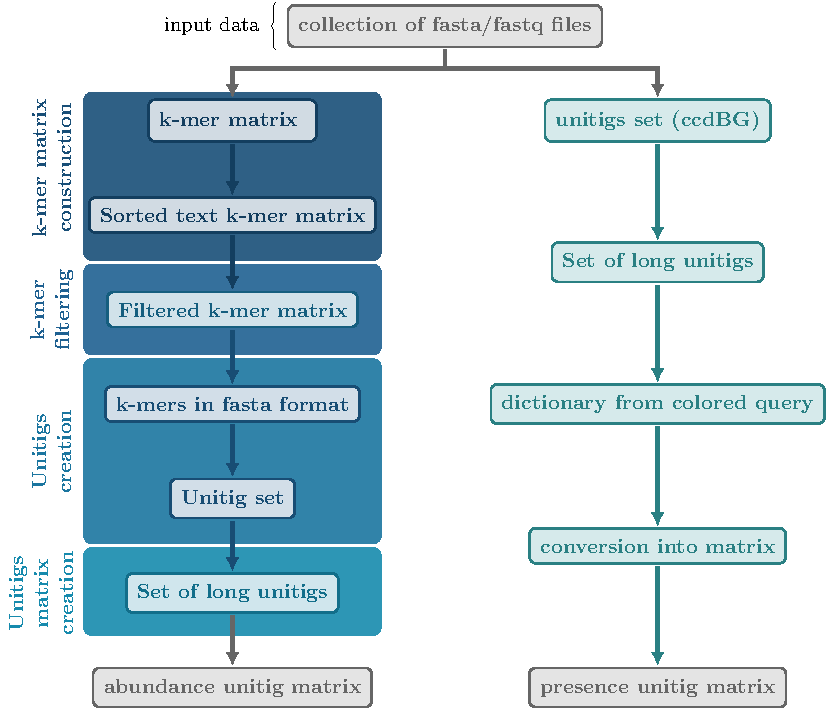
\includegraphics[width=\linewidth]{figures/kmer_methods/muset_full.pdf}
	\caption[The \muset pipeline]{Scheme representing the main steps of the \muset pipeline.}
	\label{fig:muset}
\end{figure}

\subsection{Conclusions and perspectives}
\subsubsection{Unitig matrices are pangenomes}
Matrices, although often overlooked in the pangenome community, offer a valid and valuable representation of pangenomes. Each genome can be conceptualized as a binary vector within a matrix that encodes the alleles of a pangenome graph. Both variation graphs and \ccdbgs can be used to infer presence-absence matrices, where rows represent node IDs and columns represent input samples. 
While plain text matrices may not provide the same visual representation of genome variations as graphs do, they offer distinct advantages:
\begin{enumerate}
	\item They are a more accessible starting point for downstream applications that \dbgs;
	\item bio-statistical methods and population genetics can be easily applied to this model;
	\item provide a standardized format that can be compatible with various computational tools and libraries, providing a more reliable framework for researchers to build upon. This is in distinct contrast to color representation for \ccdbgs that depend on the particular implementation.
\end{enumerate} 
The significance of \muset lies in its novel approach to generate plain text unitig matrices. Prior to the development of the \muset pipeline, abundance matrices could be theoretically generated only from paths in variation graphs. Our tool makes now possible to obtain a sufficiently precise and compact representation that enables new kind of analysis in pangenomics, transcriptomics, paleogenomics and metagenomics.\\
\subsection{Improving the method}
\muset is the first pipeline that integrates various existing and novel tools to produce unitig matrix representations of pangenomes. The \kmat software has been specifically developed for the pipeline: it implements filtering, count averaging, presence-absence steps and handles the various input/outputs. Most of the tools incorporated in \muset were instead not originally designed for this particular application.\\
While \muset's main contribution is in proposing for the first time a method to build such matrices, the current implementation has room for improvement and optimization.
The pipeline involves multiple steps in which data is written and read to disk, not for a specific design choice to ease the burden from in-memory processing, but because of subsequent steps are done by different software. Other operations are also slowing down the pipeline. Two of these that are easy to spot are: building unitigs from a file containing one \kmer per sequence in the abundance pipeline and transforming the jsonl output of \ggcat to a csv instead of using \ggcat apis to get presence values to avoid two I/O operations and dumping directly to disk the csv matrix in the presence-absence implementation.\\
Addressing these bottlenecks could yield a more optimized method to generate abundance unitig matrices that could scale to larger datasets and allow matrix-based analysis on them.
%Another, more simple, upgrade of muset would be to produce such matrices also from a variation graph to allow 

\section{Prototyping Dynamic Data structures for \kmer counting: a Rank Select Quotient Filter}
\label{sec:qf}
While abundance unitig matrices are valuable for specific genomics applications, they may not be the most efficient representation for all use-cases. In particular, some applications require rapid determination of presence or absence of specific sequences in datasets of interest. By indexing the dataset, the information is organized in data structures that enable fast data queries.\\
Sequence query in \kmer based data structures is typically performed through pseudo-alignment, a technique that involves tokenizing sequences into \kmers and querying each of them. Some data structures exploit the difference of just 1 character between subsequent \kmers to query to rapidly query multiple of them. While \cdbg or \ccdbg can be used to address this task, the graph construction is a major bottleneck and requires explicit association between each \kmer and its abundance. \\
\subsection{Brief filter data structures overview}
\kmer storing data structures imply mainly two strategies to efficiently store and retrieve them: representing \kmers as string or as hashes\cite{marchet2024kmersets}. In this work we will describe a method that stores \kmers as hashes and in particular uses structures with false positive rates. Other hash-based data structures are static or dynamic hash tables~\cite{sshash}.\\
Approximate Membership Query (AMQ) data structures, such as Bloom filters, quotient filters, and cuckoo filters, offer a more space-efficient representation of a set or multi set of elements. These data structures have become essential tools not only in computational biology but also in other domains like databases, storage systems and networks. They are termed approximate because they allow queries to return a controlled false positive value at a rate $\delta$. This means that while they always confirm the presence of an inserted item, they might erroneously return true for non-inserted items with a probability of $\delta$. This trade-off provides space savings.\\
Recent developments in the \kmer field yielded improved version of data structures that allow to store the count of elements in a dataset, instead of just reporting the absence or presence~\cite{squeakr,pandey,cqf,comin_count,sshash}. AMQs that provide this feature are termed counting AMQ or cAMQ. In the case of cAMQ, false positive values should report a count greater and not inferior to the real ones: this means that they should never underestimate the abundance of an element in the dataset. These data structures are particularly useful in many bioinformatics applications, from pangenomics to transcriptomics and metagenomics.\\
At the present moment, the main areas of improvement of such data structures are:
\begin{enumerate}
	\item latency of \memb operations. It determines the range of applications they can be used for (e.g., computer networks) and the volume of data that can be queried within a reasonable amount of time (e.g., bioinformatics). The latency is mainly influenced by:
	\begin{itemize}
		\item data locality design. Developing an architecture that reduces cache misses by storing data that might be frequently accessed together in slots that fit within the largest process cache.
		\item implementation efficiency, by carefully engineering the software for code branches, SIMD operations and multiprocessing. This is aspect is particularly important, as theoretically less efficient data structures can outperform others in practice due to optimization.
	\end{itemize}
	\item space efficiency, as it poses constraints on the computer architectures that can utilize it. Despite RAM cost declining, the more rapid growth of data requires efficient and parsimonious encoding of data to the bit level.
	\item operation range. The possibility to modify the data contained after initialization. The most useful operations are:
	\begin{itemize}
		\item incrementing elements count, or add new ones; 
		\item decrementing elements count, or removing them when their count reaches zero;
		\item enumerating elements with their respective count;
		\item automatically resize the filter when it reaches maximum capacity, avoiding the need for a priori cardinality estimation and allowing for addition of new elements.
	\end{itemize}
\end{enumerate}
A data structure that addresses efficiently all these aspects is the Counting Quotient Filter or CQF. It is based on the Rank-Select quotient filter and it uses a counting scheme to efficiently encode the count of inserted elements in the slots of the filter. This method offers reduced memory usage and faster lookup speed compared to inserting multiple times elements in a Quotient Filter to remember the counts.
\subsubsection{Filter data structures}
AMQs are often termed with the name of filter. Here I briefly describe the most common ones.
\begin{itemize}
	\item[The \textbf{Bloom filter}] is a well-known AMQ, which uses hash functions to map inserted items into a bit vector. Despite its space efficiency (one to two bytes per element for common $\delta$ values like 1/50 to 1/1000), a major drawback is it cannot be resized and doesn't support deletions. Counting Bloom filters (CBF) extend Bloom filters by using saturating counters instead of bits, enabling deletions at the cost of increased space. Scalable Bloom filters, on the other hand, maintain a low false-positive rate even when the number of items is unknown by employing multiple Bloom filters.
	\item[The \textbf{Quotient filter}] uses hashed fingerprints to manage table slots. It supports a range of operations like insertion, deletion, and resizing. It is more cache-efficient and faster than Bloom filters—though less space-efficient than CBFs—making it suitable for systems like SSDs. One downside is that its performance degrades significantly once the table exceeds 60\% occupancy.
	\item[The \textbf{Cuckoo filter}] uses cuckoo hashing. It uses two potential slots for storing each item and moves items between their alternate locations if needed, causing a cascade of movements (kicks) until a stable arrangement is achieved. This filter is fast for loockups but can suffer from poor cache performance if many kicks occur, especially when the structure becomes full.
\end{itemize}
All these implementations provide a fast lookup table where information can be stored in fixed-size slots.\\
I will focus on the implementation of the Quotient Filter, as it forms the basis of our implementation.

\subsection{Quotient Filter structure: Rank and Select}
The Rank-Select quotient filter, or RSQF, works by hashing items into a $p$-bit fingerprint $x$ and then dividing the bits into two parts: the quotient $h0(x)$ of $q$ bits and the remainder $h1(x)$ of $r = p - q$ bits. The RSQF has an array of $2^q$ $r$-bit slots that store the remainder of each item. When inserting an item, the process begins by attempting to place the remainder in the slot determined by the quotient. If the home slot is occupied, a linear probing technique is used to locate the next available slot.
To track and manage the runs (collections of subsequent slots containing remainders of a specific quotient), the the RSQF uses two metadata bitvectors:
\begin{itemize}
	\item[occupieds] it tracks which slots are currently occupied by data;
	\item[runends] indicates the end of each set of consecutive entries (or a "run") in the quotient filter.
\end{itemize}
The combination of these two bit vectors allows the RSQF to efficiently locate and manage inserted items by using rank and select operations. Specifically, the \texttt{RANK} function counts the number of occupied slots up to a certain point, and  \texttt{SELECT} identifies where in the filter a particular run ends. This allows efficient lookup, insertion, and enumeration of the data in the filter.\\
Moreover, to store the data in a cache-friendly way, the filter is structured into blocks of 64 slots. To minimize operations requiring the scan of multiple blocks when the filter is relatively full, an offsets array tracks the distance from the start of a run to where it ends, every 64 slot. Computing offsets involves scanning only small sections of the metadata (64 bits or fewer) per operation, making the filter significantly faster.\\
Each block fragments contains one offset value, 64 occupieds bits, 64 runends bits, and 64 slots for remainders data. By grouping these elements together, the system minimizes memory access and enhances cache efficiency. This structure is optimized for rapid traversal and manipulation of the filter content to enable fast membership queries and updates.\\
A scheme of how the quotient filter works is shown in figure~\ref{fig:qf_ex}. For the sake of simplicity the metadata vectors are not shown.
\begin{figure}[h!]
	\centering
	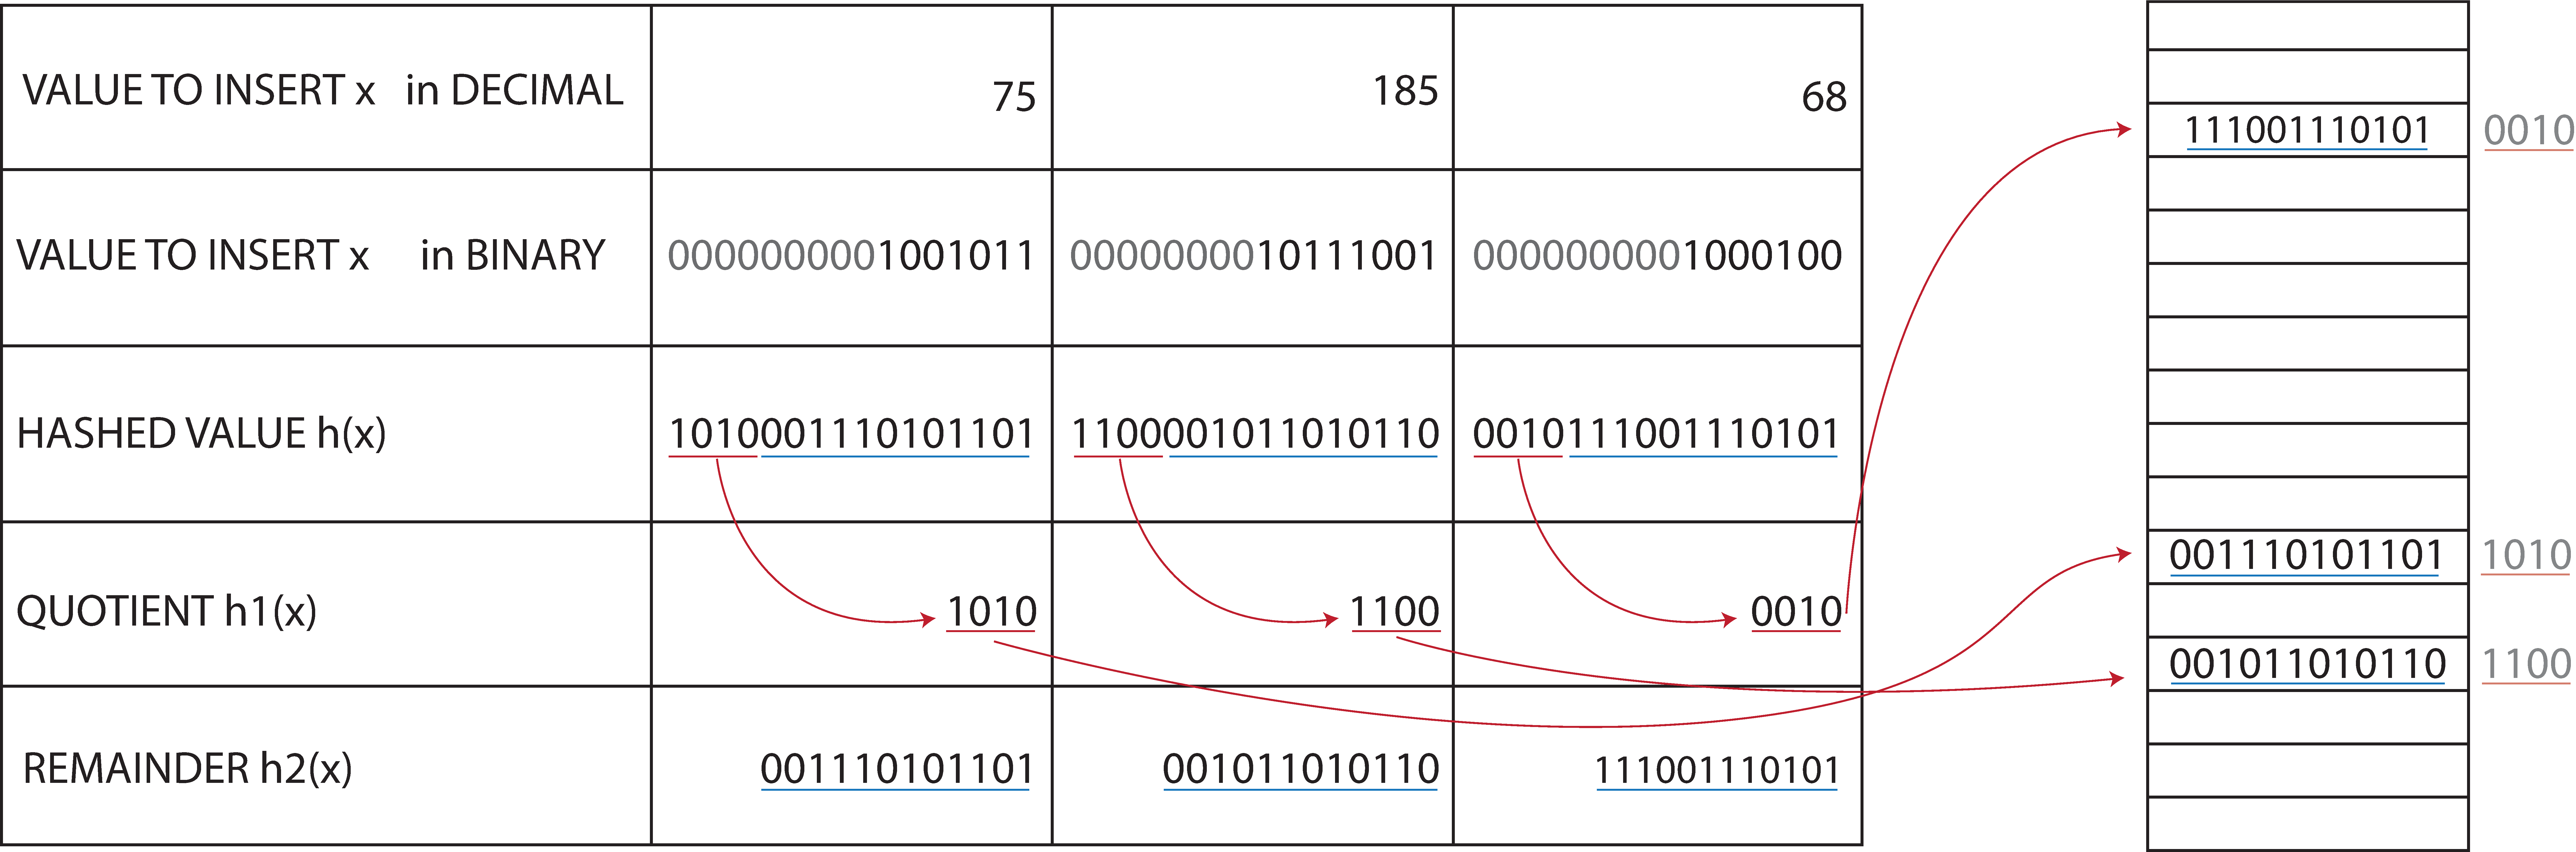
\includegraphics[width=.95\linewidth]{figures/kmer_methods/quotient_filter_export.pdf}
	\caption[Example of a quotient filter.]{Example of a quotient filter.An integer, represented in decimal form, can be expressed as a binary sequence. An unsigned 16-bit integer is composed of 16 binary digits (bits) that can store a value from $0$ to $2^{16}-1 = 65535$. To construct a quotient filter, a hash value is generated by applying some binary operations on this integer. From the computed hash value, the leftmost 4 bits are considered the quotient (although, depending on the implementation, the rightmost bits could be used instead). The remaining bits from the hash form the remainder. The remainder is stored in the filter at the position indicated by the quotient. }
	\label{fig:qf_ex}
\end{figure}
\subsubsection{Counting}
\label{sec:rsqfcount}
Counting data structures can store either exact counts or order of magnitude, depending on the application. In fields like human genomics, where count numbers are expected to be relatively low and precision is crucial, exact counts are preferred. Differently, in fields like metagenomics, where skewed abundance is more probable, an estimate of the count is often sufficient.\\
Counts can be stored using three different strategies. In all cases, the reminders associated with a certain quotient are stored in monotonic order within the data structure.
\begin{enumerate}
	\item  a count can be encoded as the number of times a reminder is inserted into consecutive slots. This is the most basic implementation and in most cases the least space-efficient one. The data structure occupation is directly related to the total number of counts in it, making poor use of the bits in the slots.
	\item a count $N$ of a reminder $R$ can be encoded into multiple consecutive slots as follows: 
	\begin{itemize}
		\item if $1 <= N <= 2$, than the reminder $R$ is inserted $N$ times;
		\item else $K = C - 2$ can be encoded into a sequence of slots. The boundaries are flagged by two remainders $R$. The slots in between store the count $K$. To signal that the slots are used as counter, the count elements break the monotonicity just after the first remainder.
		%The encoding uses the slots in between to store the actual value of the count $K$. If $K$ is greater than $R$, a 0 is placed just after the first reminder to signal that the next slots are used for encoding, else not as the monotonic insertion of the reminders would implicitly flag the count. If $K$ is greater than the max value that can be encoded in the $r$ bits of a slot (i.e. $2^r -1$), it is encoded as a sum of the slots containing the count. 
	\end{itemize}
	This approach uses at least 3 slots for $n>2$ and, while more efficient than the first, is still inefficient for low count values.
	\item another way of storing $c$ is reserving $m$ extra bits for every slot to encode in it the count associated to the remainder. As this method adds $2^q * c$ bits the choice of $c$ should be calibrated for the suited application. 
\end{enumerate}

\subsection{Developing a new library for a Quotient Filter}
The pre-existent implementation of the CQF is efficient but has several limitations. It represents an immutable object, limiting experimentation with different models based on the Rank-Select Quotient Filter or the Counting Quotient Filter. It lacks dynamicity due to static allocation of the table and does not address issues related to the filter's toricity when accommodating new elements.
To overcome these limitations, we decided to re-implement the data structure with key improvements.\\
The new data structure explicitly manages the filter's toricity, addressing cases where the final part of the filter is filled with data and new insertions push elements to the beginning of the filter. This means that there is no logical start or end of the table, as elements can be moved from the last slot to the first as continuation of the filter.\\
It automatically resizes when reaching the imposed threshold of maximum occupancy by doubling the size of the table. This feature allows for continuous insertion of new elements.\\
It supports the enumeration of inserted elements.\\
The filter is designed in a modular structure, so that the basic RSQF data structure serves as a building block for different applications.\\
The developed data structure allows for the creation of models that are:
\begin{itemize}
	\item exact (when no space trade-off is chosen) or approximate;
	\item capable of handling exact or approximate counts;
	\item capable of handling different count encoding;
\end{itemize}
The data structure is layered as follows:
\begin{itemize}
	\item[\textbf{Low Level}] comprises agnostic operations in the data structure such as
	\begin{itemize}
		\item setting a specific slot to a certain value. The value can be a remainder, count or combination of the two. It can also be any metadata as it only imposes bits to a certain region of memory corresponding to a slot;
		\item clearing of a slot to zeros for removals of elements from the filter and shifting operations;
		\item reading the value from specific slots;
		\item shifting slots by a certain amount $z$. Slots starting at position $x$ to $y$ are moved between positions $x+z$ and $y+z$ modulo the length of the filter. This operation is needed when a new element has to be inserted in an already occupied position. By shifting right of $z$ slots the already set slots, the position $x$ to $x+z-1$ are therefore free to accommodate new elements or counts;
		\item metadata operations for setting to 1 or to 0 the occupied and runends bits in their bitvectors;
		\item updating the offset vector to track of runs.
	\end{itemize}
	\item[\textbf{Medium Level}] it comprises operation to insert,removing and querying elements without explicitly caring about bit-level operations. They implement a RSQF data structure.
	\begin{itemize}
		\item addition of an element to the data structure;
		\item removal of an element from the data structure;
		\item query of an element from the data structure;
		\item metadata handling in each of the aforementioned operations.
	\end{itemize}
	\item[\textbf{High Level}] it comprises operations built on top of the RSQF layer and described a CQF.
	\begin{itemize}
		\item extended addition and removal to allow for multiple slots altogether;
		\item functions to encode and decode counters, as described in point 2 of section~\ref{sec:rsqfcount};
		\item query operations using specific linear probe, recognizing the start and end of a counter.
	\end{itemize}
	\item[\textbf{Application Specific}] functions specific for handling input, output and resize.
	\begin{itemize}
		\item \kmer hashing.
		\item initialization of the data structure;
		\item enumeration of elements within the data structure;
		\item dynamic resizing of the data structure, including element enumeration, filter size doubling, and element reinsertion;
	\end{itemize} 
\end{itemize}
This implementation has been developed as both a library and standalone software, offering flexibility in its application.
\subsubsection{Allowing multiple types of counts: CQF and BQF}
While the primary focus was on re-implementing a Counting Quotient Filter (CQF) from the Rank-Select Quotient Filter (RSQF) implementation, the basic structure with low to mid-level operations and application operations can be used to build other models on top of the RSQF. Victor Levallois has successfully implemented another data structure called the Backpack Quotient Filter (BQF), which uses the count encoding presented in point 3 of the previous section on RSQF counting methods~\ref{sec:rsqfcount}. Instead of using other slots to encode the counter, it reserves a pre-defined amount of bits in the remainder to store the approximate count:this is done at the expense of some precision~\cite{bqf}.\\
The successful implementation of the BQF demonstrates the flexibility and extensibility of the proposed architecture in order to handle different kind of counts.

\subsubsection{Handling toricity}
A crucial property of the filter, overlooked in the original CQF implementation, is the handling of specific edge cases related to its toroidal structure. Runs of reminders (or counts or combinations of both) associated with the same quotient are stored contiguously in monotonic order. This storage must be done in increasing slot ID order. When two elements with the same quotient are added to an empty filter, the slots used are the one associated with the quotient and the one \emph{on the right}(i.e., the slot associated with quotient+1), and so on.\\
A challenge arises at the \emph{rightmost} or final part of the filter. When new elements are added, it's likely that at some point, a slot should be pushed to the next element after the final slot. To address this issue, the filter is implemented with a toroidal structure, meaning the slot following the last slot is the first slot of the filter. This property eliminates problems associated with filling the filter in the final slots by imposing equal properties to all slots in the filter.\\
Implementing the filter with this characteristic is non-trivial, as the toroidal property requires different handling of all comparisons within functions and shifting operations. It necessitates careful consideration of edge cases and boundary conditions to ensure correct behavior when operations wrap around from the end to the beginning of the filter.\\
This toroidal implementation enhances the robustness and efficiency of the filter, allowing for more uniform utilization of the entire data structure and eliminating potential bottlenecks that could occur at the boundaries of a linear structure. Figure~\ref{fig:cqf_toricity} shows how the toroidal property works in a case of insertion where the final part of the remainder vector is already full.
\begin{figure}[h!]
	\centering
	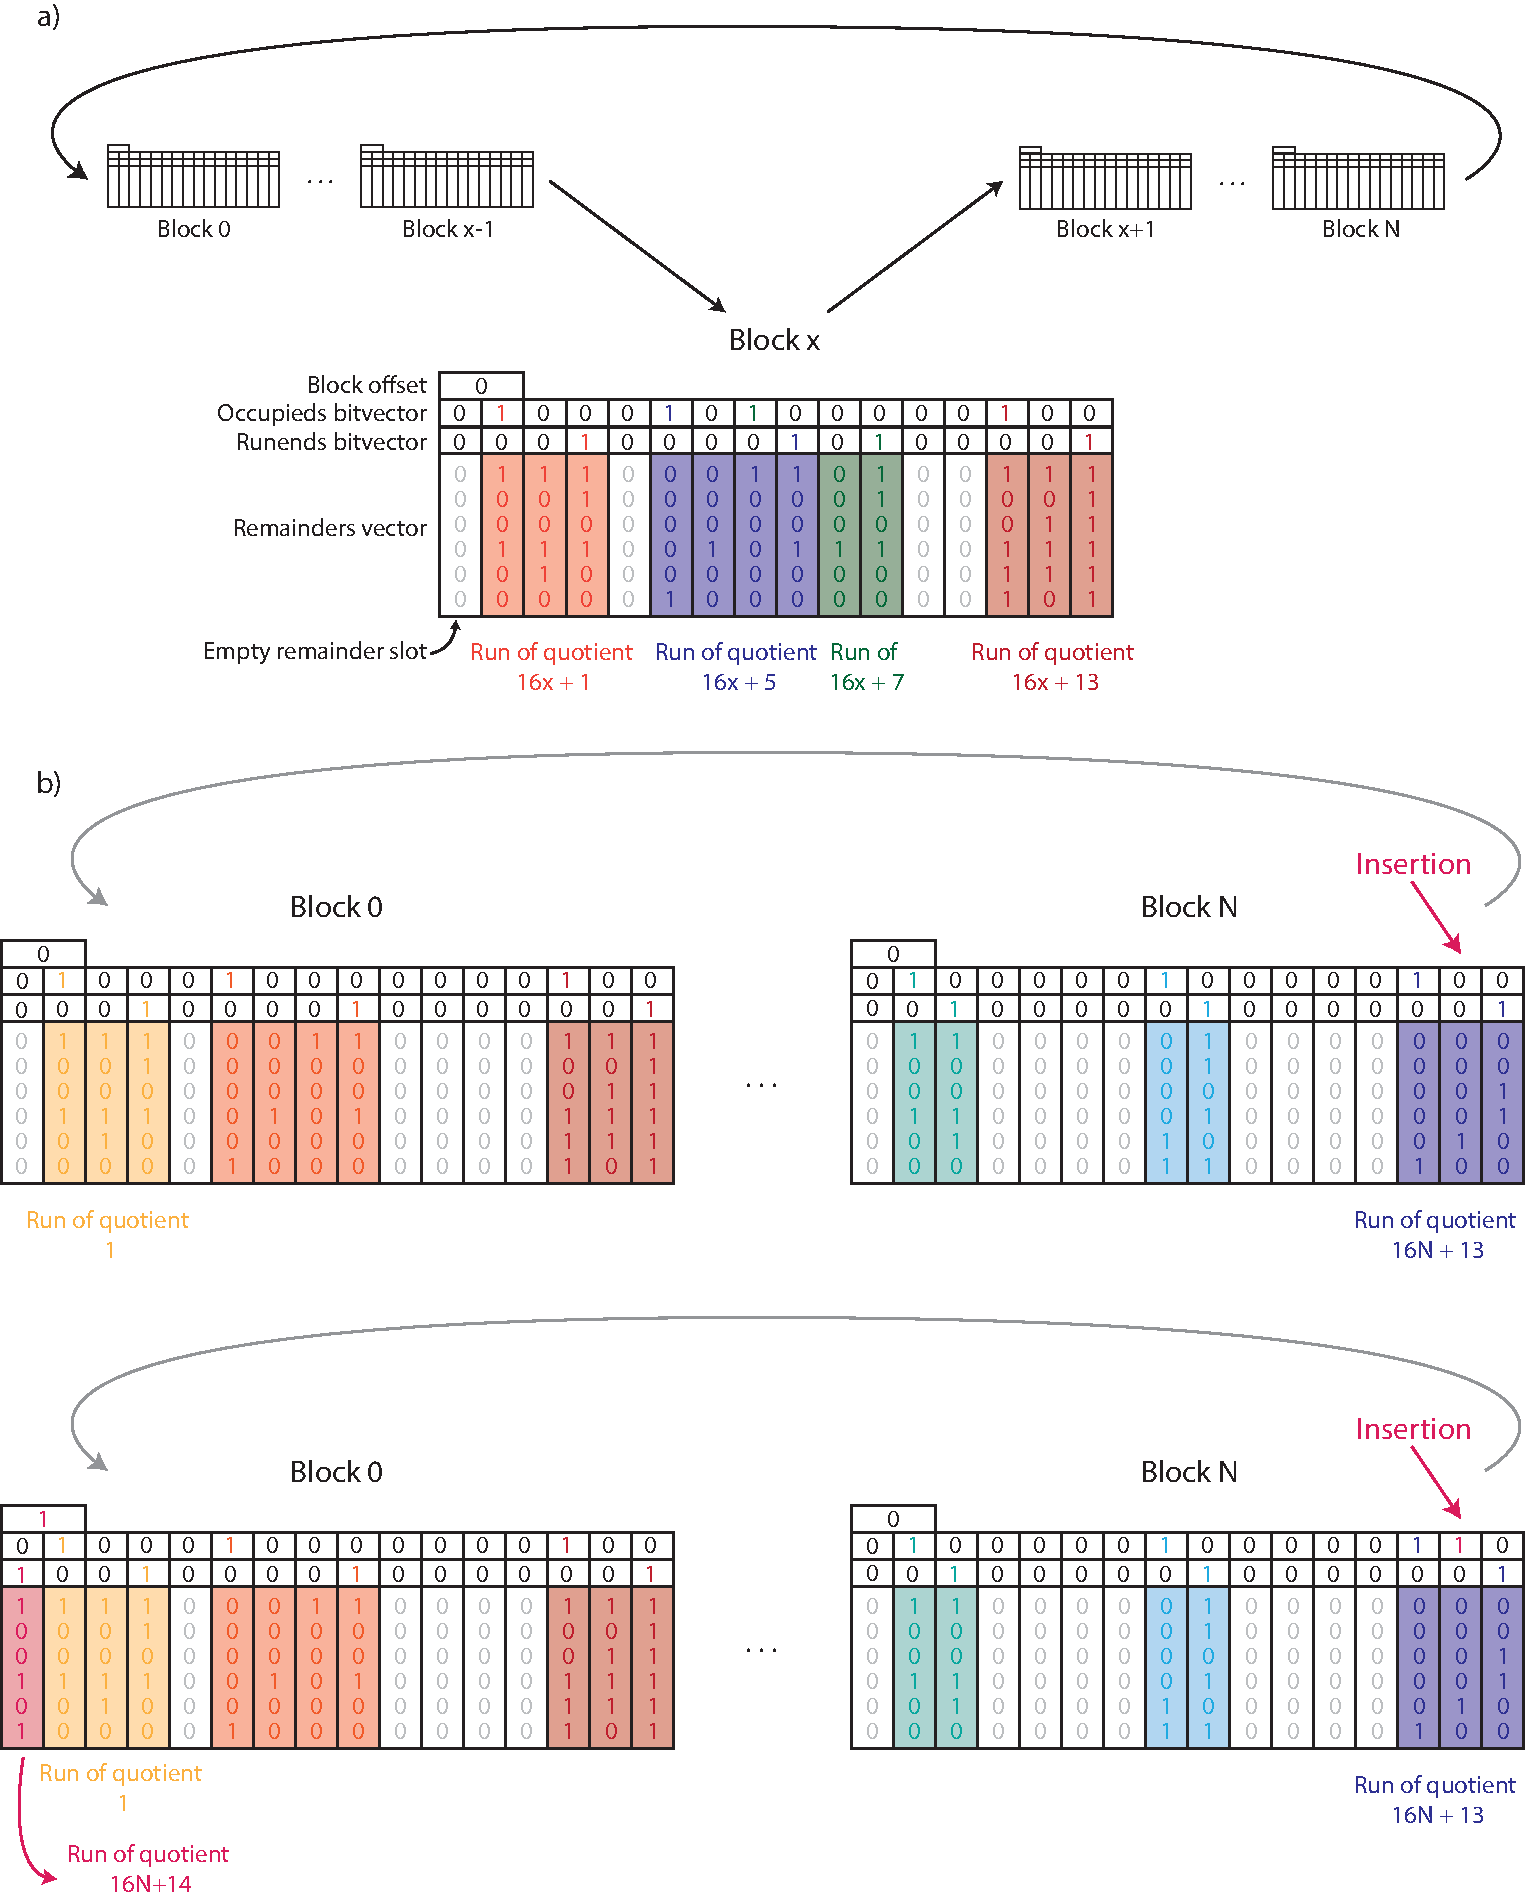
\includegraphics[width=\linewidth]{figures/kmer_methods/cqf_toricity_export.pdf}
	\caption[The RSQF data structure scheme and toroidal property]{a) Scheme of the RSQF data structure partitioned into 16 elements blocks. Along with the remainders vector, each block consists of the correspondent block of occupieds and runends bitvectors and one offset value. When elements associated to a certain quotient (here $16*x + 7$) cannot be stored in the relative slot because it is already used by another run, they are placed into the next contiguous available slots.\\
	b) example of toroidal insertion. One remainder associated to quotient $16*N + 14$ is inserted in the already partially filled data structure. Since there are no free slots in the final part of the remainder vector, the next available free slot is at the beginning of the vector. The first slot of the vector, which was free, is then filled with the remainder. Metadata bits are then updated. The occupied bit of the quotient $16*N + 14$ is set to 1. The runend at position 0 is then set to 1 and this updates the offset.} 
	\label{fig:cqf_toricity}
\end{figure}

\subsubsection{Dynamic resizing strategy}
The proposed implementation of the filter eliminates the need for a priori computation of the \kmer set cardinality (and estimating the slots used by the counts), allowing for direct data insertion. To prevent failure when the number of inserted elements exceeds capacity, a dynamic resize and reallocation strategy is implemented. A specific counter is incremented each time a slot is used in the filter. This counter keeps track of the slot occupancy ratio: when the number of occupied slots reaches 95\%, the insertion process is paused and the resize operation is initiated. The process operates as follows: 
\begin{enumerate}
	\item Enumeration: all stored elements (with their counts) are enumerated. These are temporarily stored in a hash table, with the element as the key and the count as the value. The enumeration is done by linear probing the entire filter. Each occupied metadata bit is sequentially scanned. When a bit is set to one, the probe looks for the corresponding run of remainders in the filters and proceeds to enumerating all the elements (composed of the combination of quotient and remainder) with their counts. When the entire occupieds bitvector is scanned, the enumeration ends.
	\item Parameters update: the size of the quotient is increased of one and the size of the remainder is decreased of the same amount. By adding 1 bit to the quotient, the number of index-able and insert-able elements doubles. All other internal values depending on quotient or reminder are updated. The occupancy counter is set to 0.
	\item Re-instantiation of the vectors: the remainder vector and the metadata vectors are doubled in size.
	\item Insertion of elements in the new filter. The elements are fetched from the hash table and inserted back in the filter.
\end{enumerate}
The dynamic resizing allows for flexible use of the data structure without prior knowledge of data size and ensures efficient space utilization by growing only when necessary. However, this his process produces a temporary spike in memory, by having at the same time the map containing the enumeration and the newly doubled filter.

\subsubsection{Using the Fimpera scheme to reduce space}
The size of a RSQF data structure is given by $2^q * (r + m )$ bits, where $m\sim 2.125$ metadata bits (along with some other relatively negligible overhead). This suggests that if there were a way to store nearly the same input information while reducing $r$, it would yield substantial space savings and enable the use of the data structure on larger datasets. T To achieve this goal, both the CQF implementations has been developed also with the Fimpera scheme incorporated~\cite{fimpera}, like the BQF.

Fimpera operates by splitting each \kmer into smaller \emph{s-mers} and storing them in the filter, each with the \kmer count. The \kmer abundance can thus be retrieved through its constituent \emph{s-mers}, as the presence of a\kmer implies the presence of all its constituent \emph{s-mers}.\\
This approach has been demonstrated to significantly reduce the false-positive rate by an order of magnitude without generating false negatives or underestimating \kmer abundance~\cite{fimpera}. In this context, Fimpera is used to reduce the dimension of the filter without increasing the false-positive rate, as storing smaller hashes from \emph{s-mers} results in a smaller $r$.

To estimate the correct abundance of a \kmer, the smallest count among its constituent \emph{s-mers} is used.
The major drawback of this scheme is the loss of the \kmer enumeration feature, as only the \emph{s-mers} can be retrieved. However, the dynamic resizing of the data structure is preserved as only \emph{s-mers} are required to be remembered.

This approach may introduce false positive \kmers: \kmers that are non present in the original dataset but are composed of \emph{s-mers} found in other \kmers are going to be reported as present. As this is a joint probability, it is the produce of each independent probability, becoming very low when $s$ is sufficiently large. The $s$ parameter must be chosen as a trade-off between space efficiency and false positive rates. For the BQF, this has been estimated as under $10^{-5}\%$ with $s > 20$ when $k = 32$.

This Fimpera-enhanced implementation offers a novel approach to improving the space efficiency of RSQF-based data structures while maintaining acceptable error rates and proves the flexibility of the proposed implementation.

\subsection{Conclusions and perspectives}
The proposed implementation of a prototype quotient filter has demonstrated considerable flexibility in its approach to storing \kmer abundances. This adaptability is a key feature that sets it apart from more rigid data structures and opens up new possibilities for genomic data analysis.\\
It could also incorporate additional metadata, which would extend its functionality beyond a conventional cAMQ. For instance, color information would be greatly useful for specific pangenomics applications. However, this extension is non-trivial due to the memory-intensive nature of color storage and encoding. An interesting direction could use of Shannon coding for colors. When the filter undergoes multiple resizes, each resize operation can be used to evaluate the distribution of contained colors. The result of this evaluation could be used to inform an adaptive encoding strategy where frequently occurring colors are represented with fewer bits, while less common colors are encoded with into large values. Such an approach would optimize the space-color information trade-off dynamically.\\
Despite its new features, this implementation has not yet found its way to a standalone publication. The current CQF implementation (without Fimpera) exhibited slower performance compared to the original, more optimized version. This performance disparity highlights the challenges providing implementations with new features without impacting computational efficiency.
Nevertheless, there is value in prototyping data structures that offer greater customization potential for specific applications, as they provide guidance for the evolution of more flexible and adaptable data structures.\\
Finally, the BQF implementation, based on this RSQF model, has been presented at RECOMBseq~\cite{recombseq} conference and will be soon published in the associated journal~\cite{bqf}.

\section{Prototyping Dynamic Data structures for \kmer counting: Super\kmer sorted list}
\label{sec:skmers}
This chapter has shown that there's no one-size-fits-all approach to represent \kmers efficiently. The most suitable method depends on the specific application. When comparing two datasets, for instance, one can enumerate all \kmers for each set and store them in sorted lists. The difference between sets can then be estimated using a set metric (like the Jaccard index) that accounts for \kmer differences in the lists. This process works well with sorted lists. Sorted \kmer lists also offer a reasonably fast representation for single \kmer queries without indexing. Binary search has query time $O(log{N})$, where $N$ is the cardinality of the set.\\
While not indexing the data provides slower data structure insertion time, using sorted lists has the advantage of requiring less space. A map index has $O(1)$ time for each insertion, leading to $O(N)$ when inserting $N$ elements. Sorting a list, when data is assumed random and without any supplementary hypothesis, requires $O(Nlog{N})$ time, if comparisons are performed. Using a list instead of a more complex data structure, like the QF, provides a more compact representation of the data in memory, as the list has no overhead: it does not uses empty slots, metadata vectors and additional variables. The size of the data structure is only the size of the raw data: not external bits of information are added, even if information is gained compared to the input through the sorting.\\
Instead of storing just \kmers, an encoding can be used to group together overlapping \kmers and save space. The \kmer research community has explored several space compression by encoding them within string sets. The idea is to construct string sets that contain all enumerated \kmers and nothing else. Recent models include unitigs, eulertigs, simplitigs and super\kmers~\cite{marchet2024kmersets}.\\
We then propose a novel data structure that combines the encoding of \kmers into super\kmers for space savings and a sorted list structure for relatively quick non-indexed \kmer queries. It therefore can be termed as super\kmer sorted list.\\
Super\kmers are sequences of adjacent \kmers that share the same minimizer. They generate a partition of the \kmer set, allowing for space savings and parallelization. Although they are a string representation, they are often used in hash-based methods as they are based on hashed minimizers. Another property of using super\kmers in the sorted list is that, since consecutive \kmers are close, they can be queried together with great computation time savings. To query, the algorithm locates the super\kmer linked to the queried \kmer minimizer and checks for the \kmer within the super\kmer.\\
Implementations like \blight~\cite{blight} and \ssh~\cite{sshash} use Minimal Perfect Hash Functions (MPHF) to facilitate mapping of minimizers to their corresponding super\kmers. The problem of using MPHF is that they generate a static dictionary that cannot be updated~\cite{smsketch}, forcing the data structure to be static. By using sorted superk-mer lists, we can instead provide dynamic updates.

\subsection{Super\kmer sorted lists: Input ad output}
The super\kmer sorting algorithm we propose is part of a larger super\kmer based data structure I contributed to. For brevity, we;ll omit the full details of this structure. \\
Our algorithm takes any source of \kmers and processes it to produce an enumeration of super\kmers that are then sorted into a list for efficient lookup.\\
While this method can enumerate the sorted super\kmers in text format, all the operations are done in binary space after hashing the \kmers. This approach provides space efficiency to represent the \kmers in memory and and fast machine operations to compare and modify the data.\\
The next sections provide a detailed overview of the sorting steps form the enumeration of super\kmer from the input data.

\subsection{Super\kmer list model}
To better grasp the sorting algorithm's steps, it's useful to conceptualize the super\kmer list as both a succession of string-representing objects and a matrix. This matrix is defined by two parameters: $N$, the number of enumerated super\kmers, and $M$, the maximum theoretical length of a super\kmer, where $M = 2k - m$ ($k$ = \kmer length, $m$ = minimizer length). In the matrix model, rows represent distinct strings, while columns identify specific positions within the super\kmer. An horizontal position in the matrix (column) corresponds the suffix size for the \kmer, with suffix being the number of nucleotides after the minimizer. Figure YYY shows the equivalences between these two models.\\
Most algorithm steps can be viewed as operations on the matrix columns. A key aspect of this model is that a specific position in a matrix therefore represent the presence or absence of a \kmer in the data structure.

\subsection{Sorting \kmers from the same matrix column}
\label{sec:skmersorting}
In order to allow $O(log{N})$ queries using binary search, \kmers have to be sorted by columns. This is because when a \kmer is queried against the data structure, the process is divided in two steps: it first computes the minimizer position in the \kmer to identify the column in which the \kmer can be found; it then queries the column using binary search to check if the \kmer is present or not.\\
for this reason, the sorting algorithm initial step produces a sorted list of super\kmer IDs for each matrix column. The sorting is based on comparing valid \kmers at the column position using the \kmer hash value as the ordering function. Lower hash values precede larger ones.\\
The process in each column is divided into three main steps. First, it scans the input super\kmers to select IDs of those with a valid \kmer at the column position. Then it orders the selected list by comparing the \kmer hashes. Finally, it returns the list of sorted super\kmer IDs.\\
This processing is applied to every column of the matrix and can be parallelized as columns are independent.

\subsection{Construction of overlap lists between consecutive columns}
\label{sec:skmeroverlap}
The next step in the algorithm focuses on detecting overlaps between consecutive columns. For each pair of adjacent columns, we aim to identify where the $k-1$ suffix of a \kmer in the first column overlaps with the $k-1$ prefix of a \kmer in the subsequent column. This process is performed independently for each pair of consecutive columns. This process can be divided into several steps. First, it inserts the $k-1$ prefixes of the \kmers of the second column in a hash table with the prefix as key and the super\kmer ID as value. Then for each $k-1$ suffix computed from the first column it searches for a matching value in the hash table. If found, it inserts the pair of super\kmer IDs (one from each column) into a list of candidate overlaps. It's important to note that overlap can occur between a single element of one column and multiple elements of another column. In these cases, all possible overlaps are reported. \\
Once the scan is completed, each pair of adjacent columns will have its own list of candidate overlaps. This step is used to identify potential connections between \kmers across different super\kmers, which will be used in the next steps of the algorithm. This process can also be parallelized as it involves independent operations.

\subsection{Maximal set of overlapping \kmers: co-linear chaining}
The previous step computed all possible \kmer overlap pairs. However, to produce a properly sorted list, we must respect the ordering of \kmers in all columns. Some overlaps may be therefore incompatible due to two possible scenarios:
\begin{itemize}
	\item[a] a \kmer overlaps with multiple \kmers in the adjacent column, but can be used just once;
	\item[b] pairs that ,when visualized as edges between column positions, cross each other cannot be used together as they would violate the relative column order.
\end{itemize}
Figure YYY shows examples of invalid pairs and a maximal chain. To select the maximal set of "non-crossing" pairs from those calculated earlier, we employ co-linear chaining.\\
Co-linear chaining is an algorithmic technique commonly used in alignment algorithms. In the context of pairing shared subsequences between two sequences, it can be summarized as finding pairs of connected elements such that no "crossing" connections occur when visualized geometrically. \\
In read-to-reference sequence alignment, co-linear chaining takes pairs of maximal exact matches (MEMs) as input. It then computes a chain of pairs where the selected pairs' order aligns with their appearance in both strings, while maximizing the number of bases covered by the chain in the read. Recently, this technique has also been applied to sequence-to-graph alignment in pangenomics applications.\\
In this method context, co-linear chaining is used to resolve the compatibility issues between \kmer overlap pairs, ensuring a consistent order across columns while maximizing the number of valid overlaps. This step is crucial to produce a coherent and efficiently searchable structure.
\begin{definition}[Co-linear chaining of \kmers in the matrix]
	Given 
	\begin{itemize}
		\item two ordered lists of super\kmer ids of two contiguous columns computed as in section~\ref{sec:skmersorting}.
		\begin{itemize}
			\item $ A = \{a_1, a_2, ..., a_n\}, |A| = N $, representing the left column,
			\item $ B = \{b_1, b_2, ..., b_m\}, |B| = M $, representing the right column;
		\end{itemize}
		\item a set of tuples $ V = \{(v_1,w_1),(v_2,w_2), ..., (v_k,w_k) \}$ such as $ v_i \in A$ and $ w_i \in B$ and $(v_i,w_i)$ represents an overlap between \kmers of the two contiguous columns, as computed in section~\ref{sec:skmeroverlap};
	\end{itemize}
	The goal is to find the maximal list of tuples $ U$, with $set(U) \subseteq V$ such that 
	\begin{itemize}
		\item if $v_i \prec v_j$ in $U \land v_i=a_i, v_j=a_j \implies a_i \prec a_j$, and $b_i$ < $b_j$;
		\item $\forall v, w \in U | v_i = a_x \lor w_i = b_y \implies \nexists v_j != v_i | v_j = a_x \land \nexists w_j != w_i | w_j = b_y$.  
	\end{itemize}
	The first condition implies that the ordering of the column lists $A, B$ is respected in $U$, while the second implies that each super\kmer id from $A$ or $B$ can occur only once in the list of tuples U.
\end{definition}
This problem is solved using dynamic programming~\cite{genome_scale}.\\
The co-linear chaining process begins by sorting the tuples in $V$ based on their order in $B$. ensures that no "crossing" occurs in the $w$ ids, as $w_i = b_i: b_i \prec b_j$ will always be processed before $w_j = b_j$. To resolve ties on equal $v$ values, the ordering of $v_i = a_i$ in $A$ is used.\\
Next, we apply dynamic programming over the $A$ ids to identify the largest set of pairs where the $A$ ids form a non-decreasing sequence. The score is stored for each element $v_i$ in the list of pair. A table $C$ of length $M$ is filled, where index $j$ represents the maximum possible score using tuples from $V$ such that $(v,w) has w \in \{b_1,...,b_j\}$. For any tuple, we derive a recurrence based on whether it violates or not the aforementioned conditions. The recurrence is calculate as follows: 
\begin{equation} 
C[j] = \max_{j':w_{j'} \prec w_j} C[j'] + 1
\end{equation}
if $(v_j,w_j)$ does not overlap with $ V_{j'} \subseteq \{\}(v_1,w_1),...,(v_{j-1},w_{j-1})\}$ which is the non-overlapping subset selected in the previous step.\\
To optimize the search for the best solutions $j'$ among those already computed, we use a binary search tree. It contains the best score for each value $w \in A$. As they are maintained sorted based on $A$ ordering,it allows for $O(\log{n})$ complexity when querying for the best score. When new scores are computed, the tree can also be updated in $O(log{n})$ time. From this follows that the co-linear chaining costs $O(n\log{n})$.

\subsection{Reconciliation and final output}
After computing the lists of "non-crossing" overlaps for each pair using the co-linear chaining algorithm, the next step is to reconcile this information to produce the sorted list. To better understand the rationale of the reconciliation, this process is described using the matrix representation, where \kmers in each column are sorted from top to bottom. The reconciliation process can be divided into two main parts:
\begin{enumerate}
	\item Map creation. Using the lists of non-crossing overlaps, each \kmer in the matrix is added in a map as key, with its value being the ID of the super\kmer it will be inserted into. In the case one overlap list returns the pair (x,y) and the subsequent list returns (y,z), \kmers x, y, and z will be compacted into the same super\kmer in the sorted list and thus inserted into the map with the same value (e.g., 1). Other \kmers not to be compacted in the same super\kmer will have different values.
	\item Producing the sorted list. Each column of the matrix is assigned a pointer that tracks the row containing the next \kmer to be inserted. A \kmer or a super\kmer is inserted in the final sorted list by iterating over these pointers. If a \kmer or super\kmer has all its elements flagged by a pointer, it is inserted into the list. Ties are resolved by directly comparing the two super\kmers and inserting the one with the smallest hash first. After inserting an element, the pointers on top of its \kmers are moved to the next row. This process ir repeated until all pointer reach the last element of their column.
\end{enumerate}
By using this approach, we guarantee that the final list is sorted. The second part of the process could be done in parallel from the top and the bottom of the matrix to reduce computation time.

\subsection{Searching the list}
The sorted super\kmer list produced by the outlined algorithm enables relatively fast search without indexing \kmers, using binary search. Binary search is an efficient algorithm used to locate a target value within a sorted array: it repeatedly divides the search interval in half and compares the middle element to the target.\\
In the case of looking in a sorted array with smaller values on the left and larger values on the right, if the target is smaller than the middle element, it continues the search in the remaining the left half, if it's larger, in the right half. The process continues until the element is found or the search interval is empty.\\
The \kmer query process in our sorted super\kmer list operates as follows:
\begin{enumerate}
	\item the minimizer of the \kmers is computed and the \kmer position in a super\kmer is determined.
	\item a mask associated to that position is selected;
	\item the range of the searched list is given by $[x,y]$ and set to $[0,N]$, with $N$ being the length of the list;
	\item the binary search algorithm jumps the middle super\kmer of the range $[x,y]$;
	\item if the super\kmer does not have a \kmer at the searched position, the search moves to on to the next ones until it finds one that does;
	\item the mask is applied to the super\kmer;
	\item the resulting binary value is compared to the one of the \kmer. Here one of these 3 situations can occur:
	\begin{itemize}
		\item the masked super\kmer value is greater than the \kmer, than $[x,y]$ gets updated to $[x,y] = [(y-x/2),y]$ ;
		\item the masked super\kmer value is smaller than the \kmer, than $[x,y]$ gets updated to $[x,y] = [x,(y-x/2)]$ ;
		\item the item is found, return \texttt{FOUND} or \texttt{TRUE};
	\end{itemize}
	\item if $x = y$ return \texttt{NOT FOUND} or \texttt{FALSE}, else go back to point 4;
\end{enumerate}
The advantage of this superk-mer representation is that it allows the search algorithm to jump elements (super\kmers) and directly query specific positions (offsets) based on the minimizer position of the queried \kmer. This approach avoids linear probing of entire super\kmers.\\
Finally, the time complexity may be worse than binary search due to gaps in the elements of the matrix. Not all super\kmers are maximal, therefore some queries at specific positions may be impossible due to the absence of a \kmer. An offset is valid if the super\kmer contains a \kmer in that position, and invalid otherwise. To address this, when a lookup encounters an invalid offset, it performs a linear probe on previous or subsequent elements in the list until it finds a super\kmer with a valid offset.

\subsection{Bonus optimizations}
We propose three potential optimizations for the presented algorithm:
\begin{itemize}
	\item Adding information to guide the binary search when looking in a super\kmer at an invalid offset and having to use linear probing to find a a valid one in the neighbors. This can be achieved by filling the bits of an empty offset in a super\kmer with "synthetic" nucleotides. These synthetic nucleotides don't serve as genetic information but provide a middle value between the two closest valid offset values, informing the search direction.
	\item The current lexicographic ordering of superk-mers is suboptimal due to its bias towards homopolymers and poly-A regions. We propose an improved ordering strategy that gives more weight to central nucleotides, particularly those in or closer to the minimizer. This approach could lead to a more balanced and efficient search structure.
	\item Instead of using binary search, which compares the searched element with the middle of the remaining search space at each step, we could implement interpolation search to potentially accelerate the process. Interpolation search calculates where in the remaining space the element is likely to be, based on the values at the boundaries of the space and the searched value. If the element isn't found at the calculated position, it uses the same splitting strategy as binary search.
	
\end{itemize}

\subsection{Conclusion and future work}
This project has resulted in a prototype data structure that represents a \kmer set as a sorted list of super\kmers. The advantages of this representation include:
\begin{itemize}
	\item unlike some hashing data structures such as Bloom filters, our structure can enumerate the \kmers in the set.
	\item by compressing \kmers into super\kmers, we reduce the storage space compared to an ordered list of individual \kmers.
	\item the structure allows relatively quick direct queries without the need for indexing.
	\item it enables the addition of metadata through a separate data structure.
\end{itemize}
While this work is ongoing, our goal is to publish it shortly after the defense as a novel approach to organizing dynamic datasets using \kmers.\\
Furthermore, this prototype could serve as a pre-processing step for storing \kmers in a Quotient Filter (QF). We could utilize this tool to produce a sorted and compact \kmer enumeration for direct insertion into the filter.
This approach sheds light on the gap between space-efficient representations of \kmers as string sets and queryable structures, offering a balance of compression and functionality. The potential applications extend storage, as demonstrated by its possible use in QF preprocessing. As we continue to work on this prototype, we aim to use it as valuable building block for more complex applications in large-scale genomic data.

%\subsubsection{Possible improvements}
%As just described, the super\kmer sorted list can be queried using a variation of binary search in which, when the next super\kmer to be searched has not a valid offset, it has to linear probe the elements in the list for one that does. This slows the query operation, especially in cases where the super\kmers with a valid offset are sparse. \\
%A future improvement of this algorithm would be to mitigate this issue, by adding information on non valid offsets to direct the binary search on the right direction without doing a linear probing. This strategy can be implemented by fill the bits of the super\kmer left blank when a \kmer is not stored in an informative way.\\
%Given two super\kmers $S_1$ and $S_2$ in a super\kmer sorted list and an offset $t$. If there are $n$ super\kmers between $S_1$ and $S_2$ that do not have a valid \kmer at that position $t$ while $S_1$ and $S_2$ do. The strategy is to fill the bits not used by \kmers in the super\kmer with "fake" nucleotides that do not serve as genetic information but that help the search by giving information on where to find the queried \kmer. This can be done by filling the empty bits with an average between the value found in $S_1$ and $S_2$ at the same position, starting to fill the bits from the most significant one, for all $n$ super\kmers. Another approach would also take into account the cardinality $n$ of the elements to fill and, instead of filling all the super\kmers with the same averaged value, it would fill the $n$ elements with progressive values from $S_1$ to $S_2$.

\section{\kmer based method exploration: conclusions}
In this chapter, I have presented three distinct yet interconnected projects, each utilizing \kmer data structures to enhance genomic analysis, with a particular focus on features that can best fit pangenomics applications. These efforts also span different levels of the method development stack.\\
In \muset project, which novel contribution is a pipeline for plain text unitig matrices generation, my main contribution was on the development of the pipeline and the function of the novel accompanying software, \kmat, that produces the presence-absence matrix using \ggcat. My involvement in this project arises from the conviction that there is great need for more downstream-focused \kmer tools, as they currently lag behind variation graph-based approaches for genomics analyses. Furthermore, I consider the effort to propose standardized, text-based file formats important in helping the community build software upon stable foundations.\\
The development of the RSQF-based library and tool, while not revolutionary in concept, represents a significant addition to the bioinformatics community. This prototype offers new features such as enumeration and dynamic updates, provides a clearer description and resolution of issues like toricity, and serves as a reproducible and reusable platform for building other prototypes or tools, as exemplified by the BQF.\\
The super\kmer sorting project is a novel contribution, developed in collaboration with my supervisors. This prototype introduces a novel approach to encoding super\kmers as an alternative development direction for data structures representing \kmer sets, specifically optimized for particular applications.\\
\muset is an easy recognizable example of my effort in contributing to the development of \kmer based data structures. The RSQF and super\kmer sorting are not directly linked specifically to pangenomics, as they can serve more general purposes. Nevertheless they could be used as building blocks of more comprehensive data structures to store, process and analyze pangenomes.\\
By contributing to these different projects, I have obtained a greater understanding of the strengths and challenges of \kmer based methods. I find these experiences very valuables, as I gained a comprehensive view of the field.

\printbibliography